\documentclass[12pt,a4paper]{article}
\usepackage[utf8]{inputenc}
\usepackage{amsmath}
\usepackage{amsfonts}
\usepackage{amssymb}
\usepackage{graphicx}
\usepackage{float}
\usepackage[ngerman]{babel}
\parindent0pt
\author{Matthias Englert, Fabian Schilha, Andreas Rottach}
\title{Pflichtenheft}
\begin{document}
\maketitle
\newpage
\tableofcontents
\newpage
\section{Überblick}
\subsection{Einleitung}
Dieses Software-Projekt hat sich als Ziel gesetzt eine webbasierte, zentrale E-Learning Plattform für die Studenten der Universität Ulm bereitzustellen. Das System soll die Lerninhalte individuell für jeden Benutzer in geeigneter Form strukturieren. Des Weiteren kann jeder Anwender den Lernstoff erweitern und mit anderen darüber diskutieren. Die Lerninhalte werden in einer hierarchischen Struktur mit verschiedenen Detailebenen dargestellt, um unterschiedliche Einblicke in ein Themengebiet zu ermöglichen. Das Skript soll durch verschiedene digitale Inhalte wie Bilder, Texte oder Videos unterstützt werden. Dozenten können initiale Lehrinhalte bereitstellen, die sich im Laufe des Semesters verändern oder erweitern werden können.

\subsection{Motivation}
Zurzeit verfügt die Universität Ulm über viele Plattformen (Moodle, ILIAS, Rubikon und slc) um Vorlesungsmaterialien den Studenten bereitzustellen. Diese Plattformen sind keine echten E-Learning Systeme, da man sie nur nutzt um Dokumente wie Skripte oder Übungsblätter herunterzuladen. Außerdem gibt es als einzige Informationsquelle zum Lernen nur das Skript und keine anderen Medien wie z.B. Videos. Das Skript kann dabei nur in einer festen linearen Struktur durchgearbeitet werden. Lernen ist allerdings kein linearer Prozess, sondern ein Prozess, bei dem Informationen zu einem Netzwerk zusammengebaut werden. Dieses Netzwerk zu erweitern und immer wieder umzustrukturieren stellt den eigentlichen Lernprozess da. Bei einem linearen Skript fehlen dabei Querverweise zu anderen Quellen, falls man einen Begriff beispielsweise nicht versteht. Zu diesem Lernprozess gehört auch, dass man sich mit anderen Studenten austauscht. In den bereits vorhandenen Vorlesungsplattformen lädt jedoch jeder das Skript runter und lernt für sich allein. Es gibt keine Möglichkeit persönliche Notizen im Skript mit anderen zu teilen. Dadurch bekommt auch der Dozent keine Vorstellung davon was man im Skript besser machen könnte, sodass sich das Skript über die Jahre kaum ändert.
Mit unserem E-Learning System wollen wir diese Probleme anpacken! 

\subsection{Vision und Leitbild}
Das Ziel des Projekts ist es den Studenten für jede Vorlesung eine zentrale webbasierte Lernumgebung anzubieten. Der Dozent einer Vorlesung hat die Möglichkeit eine Veranstaltung anzulegen, auf der er dann ein initiales Skript bereitstellen kann. Durch die während des Semesters aufkommenden Diskussionen ist er in der Lage das Skript mit Hilfe der Studenten zu erweitern. Die Vorlesungsinhalte sollen dabei nicht mehr linear aufgebaut sein, sondern einzelne Teile (z.B. eine Definition oder ein Satz in der Mathematik) sollen auf Karteikarten gespeichert werden. Die Karteikarten sind hierarchisch angeordnet und zusätzlich durch Querverweise miteinander verknüpft werden, sodass ein Netzwerk entsteht. Dadurch ist es für die Anzeige beispielsweise möglich auf Vorlesungsfolien weniger Information zu packen, als ins Skript, sodass die Anzeige flexibel wird. Durch die Struktur als Netzwerk ist es für einen Student, der beispielsweise ein Matheskript liest und über den Begriff der Differenzialgleichung stößt, möglich zuerst eine kurze Definition zu dem Begriff zu erhalten. Falls dies nicht ausreichend ist, hat er die Wahl sich zwischen verschiedenen Quellen zu diesem Thema zu entscheiden. Beispielsweise könnte er auf ein YouTube-Video oder eine andere Website verlinkt werden. In dem Netzwerk ist es aber trotzdem noch wichtig dass es einen linearen Pfad gibt, der das Skript repräsentiert. Des weiteren soll ein Student zu jeder Karteikarte Notizen machen oder eine Diskussion anstoßen können. Der Student kann entscheiden, ob andere seine Notizen sehen dürfen. Um die Qualität der Diskussion beurteilen zu können, gibt es die Möglichkeit, einzelne Beiträge durch positive Bewertungen hervorzuheben. Außerdem existieren Moderatoren, die die Aufgabe haben, schlechte Beiträge zu entfernen und besonders gute Beiträge ins Skript einzuarbeiten. Die Rolle des Moderators kann z.B. der Dozent oder der Übungsleiter übernehmen.



\section{Projektkontext}
Das Software-System wird im Rahmen des Softwaregrundprojekts Wintersemester 2014/2015 im Bereich Informatik entstehen. Dies kann eventuell in den Bestehenden Lehrbetrieb der Universität Ulm eingebettet werden, so dass allen Studenten an der Universität die Möglichkeit zu diesem System angeboten werden kann.

\section{Anforderungsanalyse}
\subsection{Fachwissen (Glossar)}
\begin{tabular}{l p{10cm}}  
BEGRIFF 	 & Administrator \\ 
BESCHREIBUNG & Benutzer mit erweiterten Zugansrechten zur Systemverwaltung\\ 
ISTEIN   	 & Benutzer \\
KANNSEIN 	 & Student, Tutor, Dozent \\ 
ASPEKT   	 & verwaltet die Benutzer und deren Zugangsrechte\\
BEISPIEL 	 & Anreas Rottach(Administrator)\\
\hline 
&\\ 

BEGRIFF 	 & Dozent \\ 
BESCHREIBUNG & Person die Vorlesungen veranstaltet und abhält \\ 
ISTEIN   	 & Benutzer\\
KANNSEIN 	 & Tutor, Administrator \\ 
ASPEKT   	 & stellt das initiale Skript zur Verfügung\\
BEISPIEL 	 & Prof. Dr. Helmuth Partsch\\
\hline

&\\ 

BEGRIFF 	 & Moderator \\ 
BESCHREIBUNG & Person die Foren überwacht\\
ISTEIN   	 & Benutzer \\
KANNSEIN 	 & Administrator, Tutor, Student \\ 
ASPEKT   	 & überwacht die Gesprächsthemes in den Foren \\
 	     	 & und filtert weiter gute Lehrinhalte und Verbesserungsvorschläge heraus\\
BEISPIEL 	 & Alexander Nasaal\\
\hline

&\\ 

BEGRIFF 	 & Student \\ 
BESCHREIBUNG & Immatrikulierte Person an einer Universität \\ 
ISTEIN   	 & Benutzer \\
KANNSEIN 	 & Anwender, Administrator \\ 
ASPEKT   	 & erweitert die Inhalte des Systems\\
 	     	 & und stellt diese anderen Benutzern zur Verfügung \\
BEISPIEL 	 & Alexander Nasaal\\
\hline

//

BEGRIFF 	 & Muhahahaahah \\ 
BESCHREIBUNG & Person die Vorlesungen veranstaltet und abhält \\ 
ISTEIN   	 & Benutzer\\
KANNSEIN 	 & Tutor, Administrator \\ 
ASPEKT   	 & stellt das initiale Skript zur Verfügung\\
BEISPIEL 	 & Prof. Dr. Helmuth Partsch\\
\hline

\end{tabular}


\subsection{Systemkontext}
\subsubsection{Akteure und Anwendungsfälle}
In diesem Abschnitt werden die beteiligten Akteure identifiziert. Danach werden alle auftretenden Anwendungsfälle durch Anwendungsfalldiagrame dargestellt.
Folgende Akteue sind am System beteiligt.\\\\
\paragraph{Akteure}
\mbox{}\\
\begin{tabular}{l p{10cm}}
\textbf{Akteuer} & Benutzer \\ 
\hline \textbf{Beschreibung} & Ein Benutzer kann sich am System anmelden und für Kurse registrieren. \\ 
\hline 
\end{tabular}\\\\

\begin{tabular}{l p{10cm}}
\textbf{Akteuer} & Dozent \\ 
\hline \textbf{Beschreibung} & Ein Dozent leitet eine Veranstaltung und überwacht diese. Er erstellt ein initiales Skript und steuert, wie sich dieses weiterentwickelt. Außerdem kann er Kommentare zu Diskussionen hinterlassen. Er hat die vollständige Kontrolle über eine Veranstaltung.\\ 
\hline 
\end{tabular}\\\\

\begin{tabular}{l p{10cm}}
\textbf{Akteuer} & Moderator \\ 
\hline \textbf{Beschreibung} & Ein Moderator überwacht Diskussionen. Er überträgt gute Kommentare in den Lernstoff und verbirgt nutzlose Aussagen.\\ 
\hline 
\end{tabular}\\\\

\begin{tabular}{l p{10cm}}
\textbf{Akteuer} & Administrator \\ 
\hline \textbf{Beschreibung} & Ein Administrator hat vollständigen Zugriff auf alle Veranstaltungen und ist dafür verantwortlich, auftretende Probleme zu lösen. \\ 
\hline 
\end{tabular}\\\\

\begin{tabular}{l p{10cm}}
\textbf{Akteuer} & eMail-Server \\ 
\hline \textbf{Beschreibung} & Ein eMail-Server ist für die externe Kommunikation mit den Nutzern zuständig. Er versendet Bestätigungs-Mails oder weißt auf bestimmte Änderungen hin. \\ 
\hline 
\end{tabular}\\\\

\paragraph{Anwendungsfälle}\mbox{}\\

\begin{figure}[H]
	\centering
	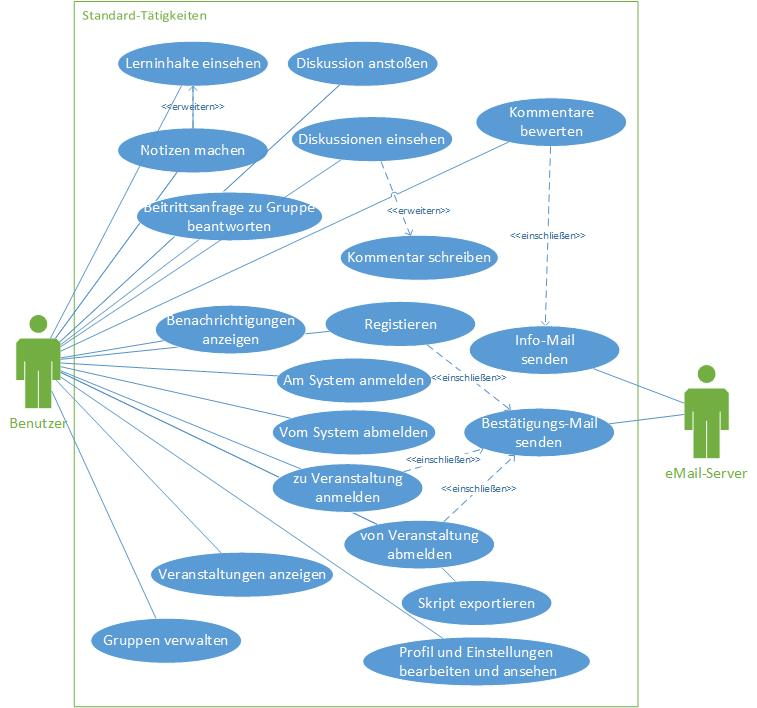
\includegraphics[width=\textwidth]{Bilder/Anwendungsfalldiagramme/Benutzer.jpg}
	\caption{Dies sind alle Aktionen die von einem Benutzer getätigt werden können.}
	\label{AwfBenutzer}
\end{figure}

\begin{figure}[H]
	\centering
	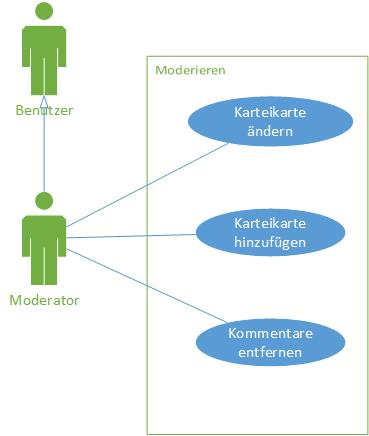
\includegraphics[width=\textwidth]{Bilder/Anwendungsfalldiagramme/Moderator.jpg}
	\caption{Der Moderator erbt alle Anwendungsfälle vom Benutzer. Er kann zusätzlich die Karteikarten und Diskussionen verwalten.}
	\label{AwfModerator}
\end{figure}

\begin{figure}[H]
	\centering
	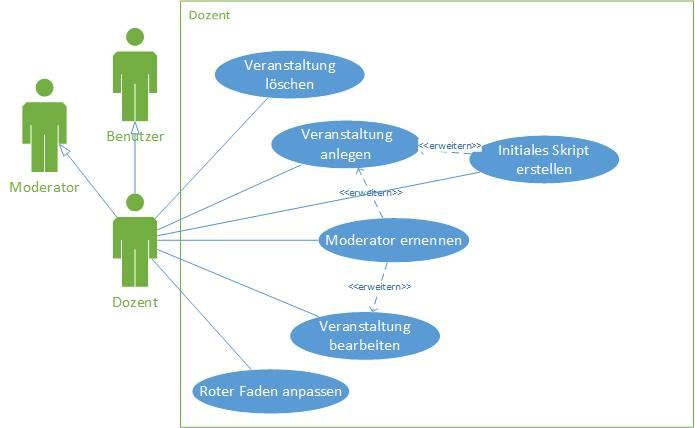
\includegraphics[width=\textwidth]{Bilder/Anwendungsfalldiagramme/Dozent.jpg}
	\caption{Der Dozent erbt alle Anwendungsfälle vom Benutzer und vom Moderator. Zusätzlich kann er Veranstaltungen verwalten.}
	\label{AwfDozent}
\end{figure}

\begin{figure}[H]
	\centering
	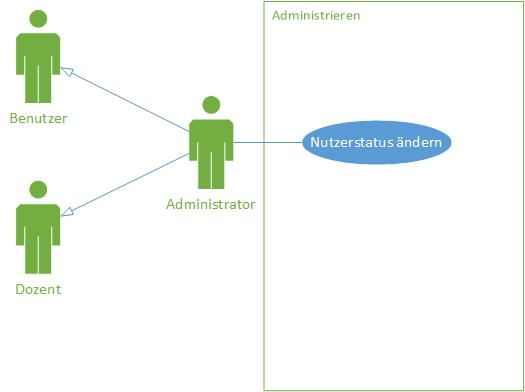
\includegraphics[width=\textwidth]{Bilder/Anwendungsfalldiagramme/Admin.jpg}
	\caption{Der Administrator erbt von allen Akteuren und hat somit alle Rechte. Er kann Nutzer in den Dozenten-Status erheben.}
	\label{AwfAdmin}
\end{figure}
\subsubsection{Szenarien}
Alle Anwendungsfälle werden durch Sequenzdiagramme beschrieben. Diese Diagramme beschreiben einen beispielhaften Ablauf einer Aktion und schließen Alternativen oder Optionales mit ein.

\begin{figure}[H]
	\centering
	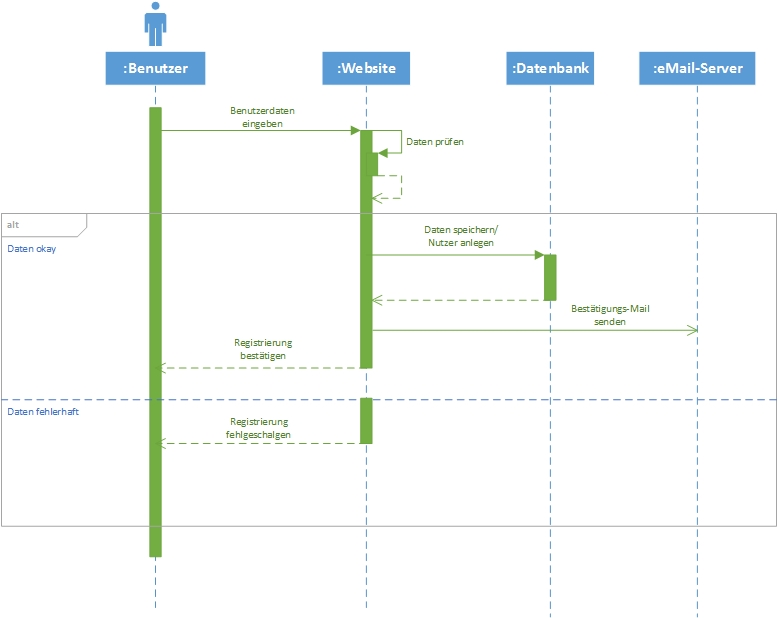
\includegraphics[width=\textwidth]{Bilder/Sequenzdiagramme/Registrierung.jpg}
	\caption{Der Benutzer registriert sich initial im System.}
	\label{SzRegistrieren}
\end{figure}
\begin{figure}[H]
	\centering
	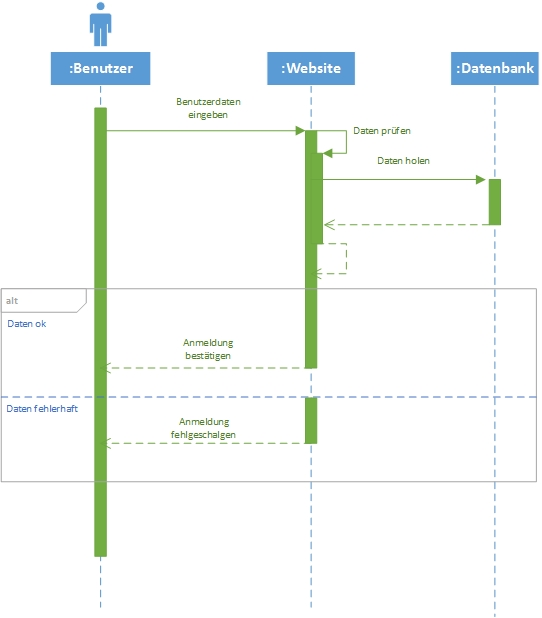
\includegraphics[width=\textwidth]{Bilder/Sequenzdiagramme/AmSystemAnmelden.jpg}
	\caption{Der Benutzer meldet am System an.}
	\label{SzAmSystemAnmelden}
\end{figure}
\begin{figure}[H]
	\centering
	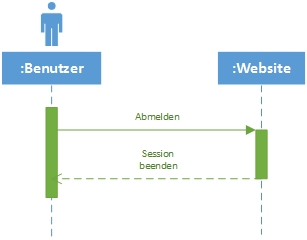
\includegraphics[width=\textwidth]{Bilder/Sequenzdiagramme/VomSystemAbmelden.jpg}
	\caption{Der Benutzer meldet vom System ab.}
	\label{SzVomSystemAbmelden}
\end{figure}
\begin{figure}[H]
	\centering
	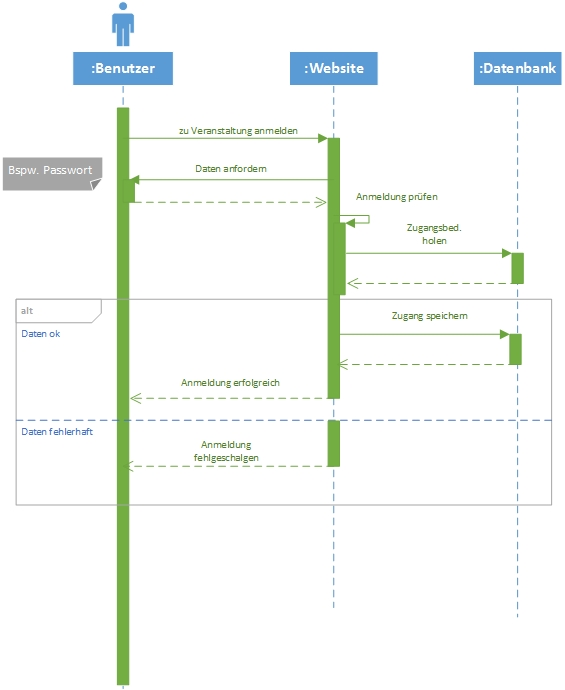
\includegraphics[width=\textwidth]{Bilder/Sequenzdiagramme/ZuVeranstaltungAnmelden.jpg}
	\caption{Der Benutzer meldet zu einer Veranstaltung an.}
	\label{SzZuVeranstaltungAnmelden}
\end{figure}
\begin{figure}[H]
	\centering
	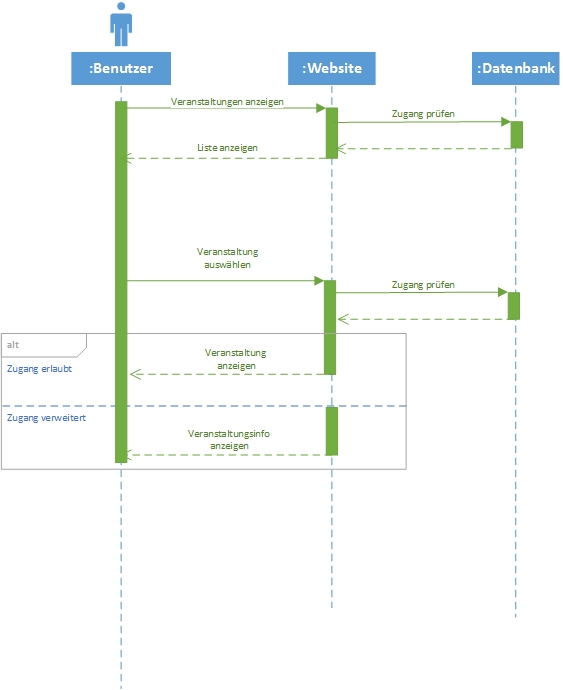
\includegraphics[width=\textwidth]{Bilder/Sequenzdiagramme/VeranstaltungenAnzeigen.jpg}
	\caption{Der Benutzer zeigt alle bestehenden Veranstaltungen an.}
	\label{SzVeranstaltungenAnzeigen}
\end{figure}
\begin{figure}[H]
	\centering
	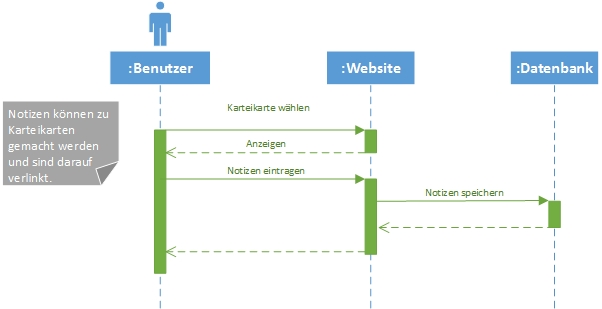
\includegraphics[width=\textwidth]{Bilder/Sequenzdiagramme/NotizenMachen.jpg}
	\caption{Der Benutzer legt eine Notiz zu einer Karteikarte an.}
	\label{SzNotizenMachen}
\end{figure}
\begin{figure}[H]
	\centering
	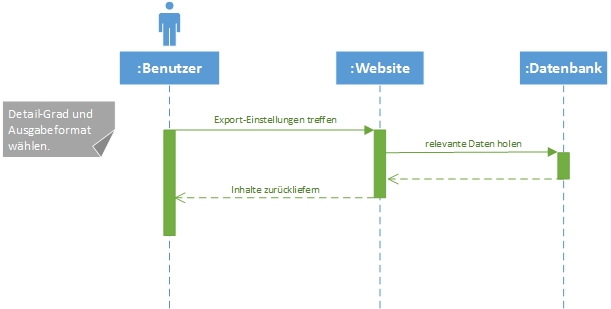
\includegraphics[width=\textwidth]{Bilder/Sequenzdiagramme/SkriptExportieren.jpg}
	\caption{Der Benutzer kann ein Skript exportieren.}
	\label{SzSkriptExportieren}
\end{figure}
\begin{figure}[H]
	\centering
	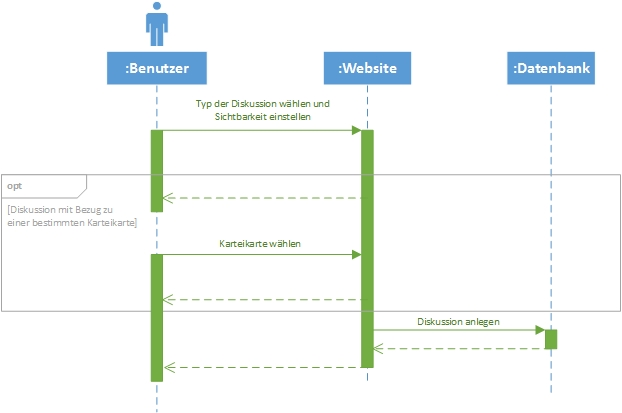
\includegraphics[width=\textwidth]{Bilder/Sequenzdiagramme/DiskussionAnstossen.jpg}
	\caption{Der Benutzer kann eine Diskussion zu einer Karteikarte beginnen.}
	\label{SzDiskussionAnstossen}
\end{figure}
\begin{figure}[H]
	\centering
	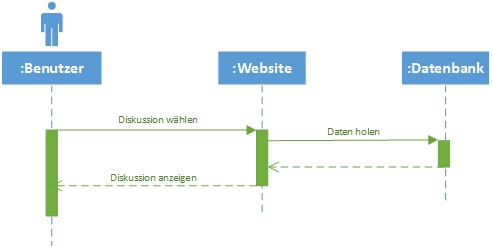
\includegraphics[width=\textwidth]{Bilder/Sequenzdiagramme/DiskussionEinsehen.jpg}
	\caption{Der Benutzer kann eine Diskussion zu einer Karteikarte einsehen.}
	\label{SzDiskussionEinsehen}
\end{figure}
\begin{figure}[H]
	\centering
	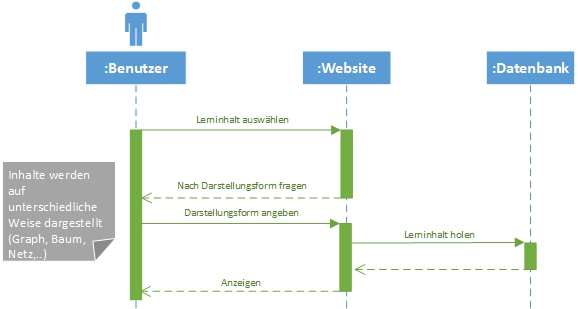
\includegraphics[width=\textwidth]{Bilder/Sequenzdiagramme/LerninhalteEinsehen.jpg}
	\caption{Der Benutzer kann eine Diskussion zu einer Karteikarte einsehen.}
	\label{SzLerninhaltEinsehen}
\end{figure}
\begin{figure}[H]
	\centering
	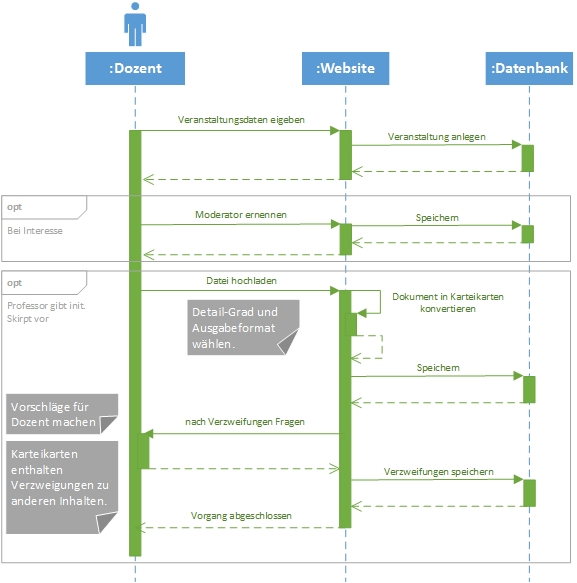
\includegraphics[width=\textwidth]{Bilder/Sequenzdiagramme/VeranstaltungAnlegen.jpg}
	\caption{Der Dozent kann eine neue Veranstaltung anlegen.}
	\label{SzVeranstaltungAnlegen}
\end{figure}
\begin{figure}[H]
	\centering
	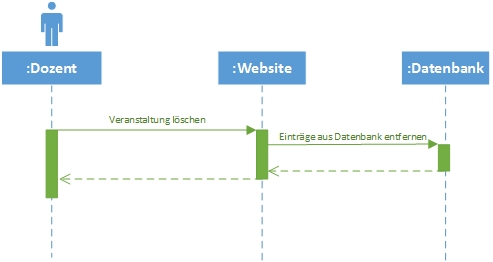
\includegraphics[width=\textwidth]{Bilder/Sequenzdiagramme/VeranstaltungLoeschen.jpg}
	\caption{Der Dozent kann selbst erstellte Veranstaltungen löschen.}
	\label{SzVeranstaltungLoeschen}
\end{figure}
\begin{figure}[H]
	\centering
	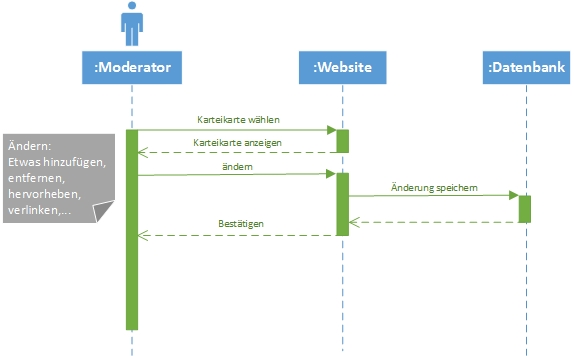
\includegraphics[width=\textwidth]{Bilder/Sequenzdiagramme/KarteikarteAendern.jpg}
	\caption{Der Moderator kann eine Karteikarte ändern.}
	\label{SzKarteikarteAendern}
\end{figure}
\begin{figure}[H]
	\centering
	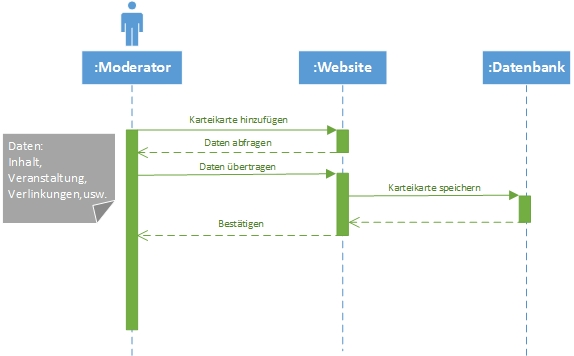
\includegraphics[width=\textwidth]{Bilder/Sequenzdiagramme/KarteikarteHinzufuegen.jpg}
	\caption{Der Moderator kann eine Karteikarte hinzufügen.}
	\label{SzKarteikarteHinzufuegen}
\end{figure}
\begin{figure}[H]
	\centering
	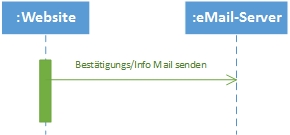
\includegraphics[width=\textwidth]{Bilder/Sequenzdiagramme/MailVersenden.jpg}
	\caption{Das System kann eine Mail an den Benutzer versenden.}
	\label{SzMailVersenden}
\end{figure}
\begin{figure}[H]
	\centering
	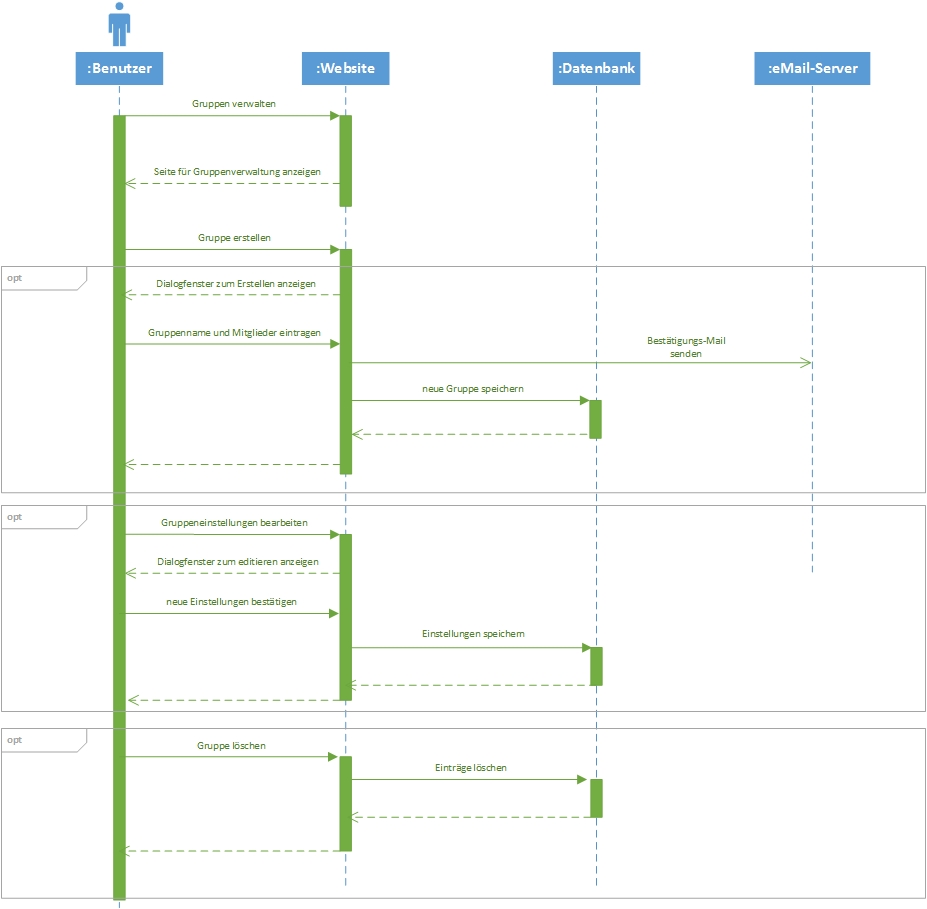
\includegraphics[width=\textwidth]{Bilder/Sequenzdiagramme/GruppenVerwalten.jpg}
	\caption{Der Nutzer kann Gruppen anlegen, löschen und bearbeiten.}
	\label{SzGruppenVerwalten}
\end{figure}
\begin{figure}[H]
	\centering
	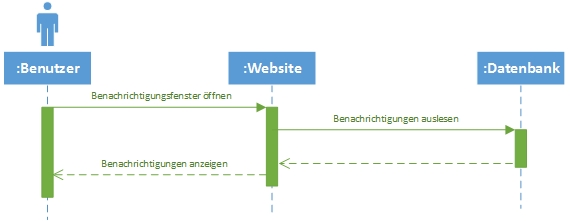
\includegraphics[width=\textwidth]{Bilder/Sequenzdiagramme/BenachrichtigungenAnzeigen.jpg}
	\caption{Der Nutzer kann seine Benachrichtigungen anzeigen.}
	\label{SzBenachrichtigungen}
\end{figure}
\begin{figure}[H]
	\centering
	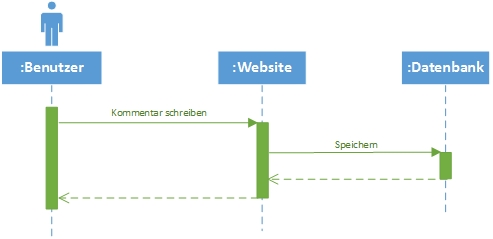
\includegraphics[width=\textwidth]{Bilder/Sequenzdiagramme/KommentarSchreiben.jpg}
	\caption{Der Nutzer kann Kommentare zu Diskussionen hinterlassen.}
	\label{SzKommentarSchreiben}
\end{figure}
\begin{figure}[H]
	\centering
	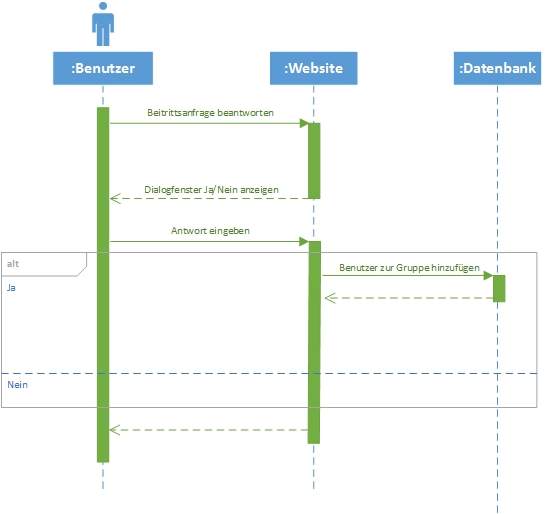
\includegraphics[width=\textwidth]{Bilder/Sequenzdiagramme/BeitrittsanfrageZuGruppe.jpg}
	\caption{Der Nutzer kann Beitrittsanfragen zu Gruppen beantworten.}
	\label{SzBeitrittsanfrageZuGruppe}
\end{figure}
\begin{figure}[H]
	\centering
	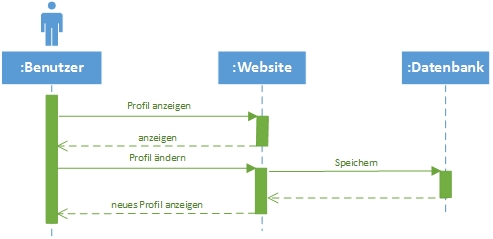
\includegraphics[width=\textwidth]{Bilder/Sequenzdiagramme/ProfilBearbeiten.jpg}
	\caption{Der Nutzer kann sein sein Profil bearbeiten.}
	\label{SzProfilBearbeiten}
\end{figure}
\begin{figure}[H]
	\centering
	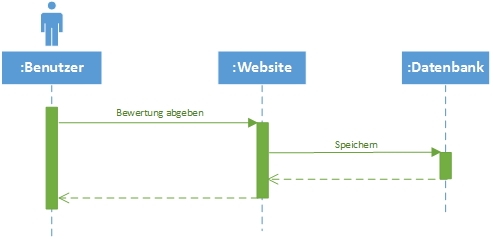
\includegraphics[width=\textwidth]{Bilder/Sequenzdiagramme/KommentareBewerten.jpg}
	\caption{Der Nutzer kann Kommentare zu Diskussionen mit positiven Bewertungen versehen.}
	\label{SzKommentareBearbeiten}
\end{figure}
\begin{figure}[H]
	\centering
	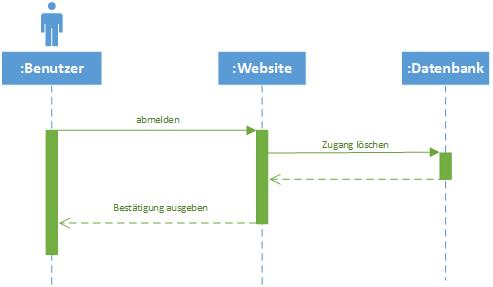
\includegraphics[width=\textwidth]{Bilder/Sequenzdiagramme/VonVeranstaltungAbmelden.jpg}
	\caption{Der Nutzer sich von Veranstaltungen wieder abmelden.}
	\label{SzVonVeranstaltungAbmelden}
\end{figure}
\begin{figure}[H]
	\centering
	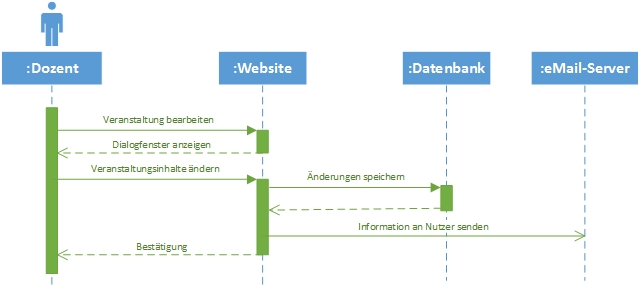
\includegraphics[width=\textwidth]{Bilder/Sequenzdiagramme/VeranstaltungBearbeiten.jpg}
	\caption{Der Dozent kann seine eigenen Veranstaltungen bearbeiten.}
	\label{SzVeranstaltungBearbeiten}
\end{figure}

\subsubsection{Systemaufgabe}
Hier werden alle Systemaufgaben, die dazugehörigen Teilnehmer und jeweils eine kurze Beschreibung aufgelistet. Außerdem wird jede Anforderung mit einer Markierung (-2 bis 2) versehen, die darlegt, wie wichtig diese Anforderung ist.

\paragraph{Funktionale Anforderungen}
\subparagraph{Benutzer - Anwendungsfall "Registrieren" (2)}\mbox{}\\

\begin{tabular}{l p{10cm}}
\multicolumn{2}{l}{\textbf{Eingabe der Daten}} \\ \hline
\textbf{Beteiligt} & Anonym, System \\ \hline 
\textbf{Beschreibung} & Eine anonyme Person kann ihre Zugangsdaten bei der Registrierung eingeben. Mit diesen Daten wird dann ein neuer Benutzer im System angemeldet.\\ 
\hline 
\end{tabular}\\\\

\begin{tabular}{l p{10cm}}
\multicolumn{2}{l}{\textbf{Registrierung bestätigen}} \\ \hline
\textbf{Beteiligt} & Benutzer, System, eMail-Server \\ \hline 
\textbf{Beschreibung} & Die erfolgreiche Anmeldung wird dem Benutzer per Dialog und zusätzlich per Mail bestätigt.\\ 
\hline 
\end{tabular}\\\\
\subparagraph{Benutzer - Anwendungsfall \glqq Am System anmelden \grqq (2)}\mbox{}\\

\begin{tabular}{l p{10cm}}
\multicolumn{2}{l}{\textbf{Eingabe der Zugangsdaten}} \\ \hline
\textbf{Beteiligt} & Benutzer, System \\ \hline 
\textbf{Beschreibung} & Der Nutzer gibt seine Zugangsdaten (eMail-Adresse und Passwort) ein. Wenn diese Daten korrekt sind, wird er im System angemeldet und eine Session wird gestartet. Andernfalls erhält er eine Fehlermeldung.\\ 
\hline 
\end{tabular}\\\\

\begin{tabular}{l p{10cm}}
\multicolumn{2}{l}{\textbf{Anmeldung bestätigen}} \\ \hline
\textbf{Beteiligt} & Benutzer, System \\ \hline 
\textbf{Beschreibung} & Das System bestätgit dem Nutzer die Anmeldung.\\ 
\hline 
\end{tabular}\\\\
\subparagraph{Benutzer - Anwendungsfall \glqq Vom System abmelden \grqq (2)}\mbox{}\\

\begin{tabular}{l p{10cm}}
\multicolumn{2}{l}{\textbf{Abmelden}} \\ \hline
\textbf{Beteiligt} & Benutzer, System \\ \hline 
\textbf{Beschreibung} & Das System beendet die Session des Nutzers.\\ 
\hline 
\end{tabular}\\\\

\begin{tabular}{l p{10cm}}
\multicolumn{2}{l}{\textbf{Abmeldung bestätigen}} \\ \hline
\textbf{Beteiligt} & Benutzer, System \\ \hline 
\textbf{Beschreibung} & Das System zeigt an, dass das Abmelden erfolgreich war.\\ 
\hline 
\end{tabular}\\\\
\subparagraph{Benutzer - Anwendungsfall \glqq Veranstaltungen anzeigen \grqq (2)}\mbox{}\\

\begin{tabular}{l p{10cm}}
\multicolumn{2}{l}{\textbf{Alle Veranstaltungen anzeigen}} \\ \hline
\textbf{Beteiligt} & Benutzer, System \\ \hline 
\textbf{Beschreibung} & Das System zeigt dem Benutzer alle verfügbaren Veranstaltungen an.\\ 
\hline 
\end{tabular}\\\\

\begin{tabular}{l p{10cm}}
\multicolumn{2}{l}{\textbf{Veranstaltungen auswählen und anzeigen}} \\ \hline
\textbf{Beteiligt} & Benutzer, System \\ \hline 
\textbf{Beschreibung} & Das System zeigt dem Benutzer die Info-Seite der Veranstaltung an, falls er nicht schon zur Veranstaltung angemeldet ist. Ist er schon angemeldet, wird ihm direkt die eigentliche Veranstaltungsseite angezeigt.\\ 
\hline 
\end{tabular}\\\\

\subparagraph{Benutzer - Anwendungsfall \glqq Zu Veranstaltung anmelden \grqq (2)}\mbox{}\\

\begin{tabular}{l p{10cm}}
\multicolumn{2}{l}{\textbf{Zu Veranstaltung anmelden}} \\ \hline
\textbf{Beteiligt} & Benutzer, System \\ \hline 
\textbf{Beschreibung} & Nachdem der Benutzer die Zugansdaten zur Veranstaltung (Passwort, falls vorhanden) richtig angegeben hat, wird die Zugangsberechtigung vom System übernommen und der Benutzer wird zur Veranstaltugnsseite weitergeleitet. Andernfalls wird ihm ein Fehler angezeigt.\\ 
\hline 
\end{tabular}\\\\
\subparagraph{Benutzer - Anwendungsfall \glqq Von Veranstaltung abmelden\grqq (0)}\mbox{}\\

\begin{tabular}{l p{10cm}}
\multicolumn{2}{l}{\textbf{Von Veranstaltung abmelden}} \\ \hline
\textbf{Beteiligt} & Benutzer, System \\ \hline 
\textbf{Beschreibung} & Das System meldet den Benutzer vom System ab und zeigt Ihm an ob der Vorgang erfolgreich war.\\ 
\hline 
\end{tabular}\\\\
\subparagraph{Benutzer - Anwendungsfall \glqq Skript exportieren\grqq (-1)}\mbox{}\\

\begin{tabular}{l p{10cm}}
\multicolumn{2}{l}{\textbf{Exportseite anzeigen und Skript wählen}} \\ \hline
\textbf{Beteiligt} & Benutzer, System \\ \hline 
\textbf{Beschreibung} & Der Nutzer bekommt eine Exportoberfläche angezeigt, auf der er den zu exportierenden Lernstoff wählen kann.\\ 
\hline 
\end{tabular}\\\\

\begin{tabular}{l p{10cm}}
\multicolumn{2}{l}{\textbf{Exporteinstellungen treffen}} \\ \hline
\textbf{Beteiligt} & Benutzer, System \\ \hline 
\textbf{Beschreibung} & Der Benutzer hat die Möglichkeit die Export-Einstellungen festzulegen.\\ 
\hline 
\end{tabular}\\\\

\begin{tabular}{l p{10cm}}
\multicolumn{2}{l}{\textbf{Skript exportieren}} \\ \hline
\textbf{Beteiligt} & Benutzer, System \\ \hline 
\textbf{Beschreibung} & Das System generiert das Dokument und bietet es dem Nutzer zum Download an.\\ 
\hline 
\end{tabular}\\\\
\subparagraph{Benutzer - Anwendungsfall \glqq Profil und Einstellungen bearbeiten und ansehen\grqq  (2)}\mbox{}\\

\begin{tabular}{l p{10cm}}
\multicolumn{2}{l}{\textbf{Profil anzeigen}} \\ \hline
\textbf{Beteiligt} & Benutzer, System \\ \hline 
\textbf{Beschreibung} & Der Nutzer kann sein eigenes Profil oder das anderer Benutzer einsehen.\\ 
\hline 
\end{tabular}\\\\

\begin{tabular}{l p{10cm}}
\multicolumn{2}{l}{\textbf{Profil bearbeiten}} \\ \hline
\textbf{Beteiligt} & Benutzer, System \\ \hline 
\textbf{Beschreibung} & Jeder Nutzer kann sein eigenes Profil bearbeiten.\\ 
\hline 
\end{tabular}\\\\

\begin{tabular}{l p{10cm}}
\multicolumn{2}{l}{\textbf{Einstellungen bearbeiten}} \\ \hline
\textbf{Beteiligt} & Benutzer, System \\ \hline 
\textbf{Beschreibung} & Das System bietet dem Nutzer eine Oberfläche um sämtliche Einstellungen festzulegen.\\ 
\hline 
\end{tabular}\\\\

\begin{tabular}{l p{10cm}}
\multicolumn{2}{l}{\textbf{Einstellungen- und Profil-Änderungen speichern}} \\ \hline
\textbf{Beteiligt} & Benutzer, System \\ \hline 
\textbf{Beschreibung} & Das System bestätigt dem Benutzer die erfolgreiche Änderung oder gibt eine Fehlermeldung aus.\\ 
\hline 
\end{tabular}\\\\
\subparagraph{Benutzer - Anwendungsfall \glqq Diskussion anstoßen\grqq (1)}\mbox{}\\

\begin{tabular}{l p{10cm}}
\multicolumn{2}{l}{\textbf{Neue Diskussion erstellen}} \\ \hline
\textbf{Beteiligt} & Benutzer, System \\ \hline 
\textbf{Beschreibung} & Jeder Nutzer kann eine neue Diskussion zu einer Karteikarte erstellen.\\ 
\hline 
\end{tabular}\\\\

\begin{tabular}{l p{10cm}}
\multicolumn{2}{l}{\textbf{Sichtbarkeit einstellen}} \\ \hline
\textbf{Beteiligt} & Benutzer, System \\ \hline 
\textbf{Beschreibung} & Der Nutzer kann beim Erstellen die Sichtbarkeit der Diskussion einstellen (Öffentlich, Veranstaltung, Gruppe).\\ 
\hline 
\end{tabular}\\\\
\subparagraph{Benutzer - Anwendungsfall \glqq Kommentare machen\grqq (1)}\mbox{}\\

\begin{tabular}{l p{10cm}}
\multicolumn{2}{l}{\textbf{Kommentar hinzufügen}} \\ \hline
\textbf{Beteiligt} & Benutzer, System \\ \hline 
\textbf{Beschreibung} & Jeder Benutzer kann, wenn er die notwendigen Rechte hat, Kommentare zu einer Diskussion hinzufügen.\\ 
\hline 
\end{tabular}\\\\
\subparagraph{Benutzer - Anwendungsfall \glqq Notizen machen\grqq (1)}\mbox{}\\

\begin{tabular}{l p{10cm}}
\multicolumn{2}{l}{\textbf{Notizen hinzufügen}} \\ \hline
\textbf{Beteiligt} & Benutzer, System \\ \hline 
\textbf{Beschreibung} & Jeder Benutzer kann, zu einer Karteikarte Notizen machen.\\ 
\hline 
\end{tabular}\\\\
\subparagraph{Benutzer - Anwendungsfall \glqq Kommentare bewerten\grqq (-1)}\mbox{}\\

\begin{tabular}{l p{10cm}}
\multicolumn{2}{l}{\textbf{Kommentar bewerten}} \\ \hline
\textbf{Beteiligt} & Benutzer, Moderator, System \\ \hline 
\textbf{Beschreibung} & Jeder Benutzer kann, wenn er die notwendigen Rechte(Sichtbarkeit) hat, bewerten. Ein Moderator kann alle Kommentare bewerten.\\ 
\hline 
\end{tabular}\\\\

\subparagraph{Benutzer - Anwendungsfall \glqq Gruppen verwalten\grqq (-2)}\mbox{}\\

\begin{tabular}{l p{10cm}}
\multicolumn{2}{l}{\textbf{Gruppe erstellen}} \\ \hline
\textbf{Beteiligt} & Benutzer, System \\ \hline 
\textbf{Beschreibung} & Jeder Benutzer besitzt Zugriff auf ein Menü, um eine Gruppe hinzufügen.\\ 
\hline 
\end{tabular}\\\\

\begin{tabular}{l p{10cm}}
\multicolumn{2}{l}{\textbf{Gruppe löschen}} \\ \hline
\textbf{Beteiligt} & Benutzer, System \\ \hline 
\textbf{Beschreibung} & Jeder Benutzer besitzt Zugriff auf ein Menü, um seine selbst erstellten Gruppen zu löschen.\\ 
\hline 
\end{tabular}\\\\

\begin{tabular}{l p{10cm}}
\multicolumn{2}{l}{\textbf{Gruppe editieren}} \\ \hline
\textbf{Beteiligt} & Benutzer, System \\ \hline 
\textbf{Beschreibung} & Jeder Benutzer hat die Möglichkeit, seine selbst erstellten Gruppen zu editieren, indem er bspw. neue Mitglieder hinzufügt.\\ 
\hline 
\end{tabular}\\\\
\subparagraph{Benutzer - Anwendungsfall \glqq Benachrichtigungen anzeigen\grqq  (1)}\mbox{}\\

\begin{tabular}{l p{10cm}}
\multicolumn{2}{l}{\textbf{Benachrichtigungen anzeigen}} \\ \hline
\textbf{Beteiligt} & Benutzer, System \\ \hline 
\textbf{Beschreibung} & Jedem Benutzer werden immer aktuelle Informationen wie eine Beitrittsanfrage zu einer Gruppe, oder neue Kommentare angezeigt.\\ 
\hline 
\end{tabular}\\\\
\subparagraph{Benutzer - Anwendungsfall \glqq Lerninhalte anzeigen\grqq  (2)}\mbox{}\\
\begin{tabular}{l p{10cm}}
\multicolumn{2}{l}{\textbf{Lerninhalte anzeigen}} \\ \hline
\textbf{Beteiligt} & Benutzer, System \\ \hline 
\textbf{Beschreibung} & Jedem Benutzer werden auf Wunsch die Lerninhalte zu einer Veranstaltung angezeigt, wenn er zur Veranstaltung angemeldet ist.\\ 
\hline 
\end{tabular}\\\\
\subparagraph{Benutzer - Anwendungsfall \glqq Beitrittsanfrage zu Gruppe beantworten\grqq (-2)}\mbox{}\\

\begin{tabular}{l p{10cm}}
\multicolumn{2}{l}{\textbf{Beitrittsanfragen beantworten}} \\ \hline
\textbf{Beteiligt} & Benutzer, Moderator, System \\ \hline 
\textbf{Beschreibung} & Jeder Benutzer kann über eine Dialog ausstehende Beitrittsanfragen annehmen oder ablehnen.\\ 
\hline 
\end{tabular}\\\\
\subparagraph{Dozent - Anwendungsfall \glqq Veranstaltung anlegen\grqq (2)}\mbox{}\\

\begin{tabular}{l p{10cm}}
\multicolumn{2}{l}{\textbf{Veranstaltungsdaten eingeben}} \\ \hline
\textbf{Beteiligt} & Dozent, System \\ \hline 
\textbf{Beschreibung} & Es gibt eine Oberfläche, wo der Dozent die Veranstaltungsdaten(Name, Beschreibung, Zugangspasswort,..) eigeben kann. Daraufhin wird eine neue Veranstaltung im System angelegt. Siehe auch Anwendungsfall \glqq Initiales Skript importieren \grqq . \\ 
\hline 
\end{tabular}\\\\
\subparagraph{Dozent - Anwendungsfall \glqq Moderator ernennen\grqq (2)}\mbox{}\\

\begin{tabular}{l p{10cm}}
\multicolumn{2}{l}{\textbf{Moderator ernnenen}} \\ \hline
\textbf{Beteiligt} & Dozent, System \\ \hline 
\textbf{Beschreibung} & Der Dozent kann für seien Veranstaltungen Moderatoren angeben.\\ 
\hline 
\end{tabular}\\\\
\subparagraph{Dozent - Anwendungsfall \glqq Initiales Skript erstellen\grqq (1)}\mbox{}\\

\begin{tabular}{l p{10cm}}
\multicolumn{2}{l}{\textbf{Importseite anzeigen und Skript hochladen}} \\ \hline
\textbf{Beteiligt} & Dozent, System \\ \hline 
\textbf{Beschreibung} & Der Dozent bekommt eine Importoberfläche angezeigt und lädt ein Dokument hoch. Nachem der Dozent die Import-Einstellungen angegeben hat, konvertiert das System dieses Dokument in die Karteikarten-Repräsentation, erstellt den initialen roten Faden und bietet die Möglichkeit zusätzliche Verlinkungen einzufügen.\\ 
\hline 
\end{tabular}\\\\
\subparagraph{Dozent - Anwendungsfall \glqq Veranstaltung bearbeiten\grqq (0)}\mbox{}\\

\begin{tabular}{l p{10cm}}
\multicolumn{2}{l}{\textbf{Veranstaltung bearbetien}} \\ \hline
\textbf{Beteiligt} & Dozent, System \\ \hline 
\textbf{Beschreibung} & Der Dozent kann seine eigenen Veranstlatungen bearbeiten, indem er neue Moderatoren hinzufügt, andere löscht, optionale Features ein oder aus schaltet oder die Veranstaltungsbeschreibung ändert.\\ 
\hline 
\end{tabular}\\\\
\subparagraph{Dozent - Anwendungsfall \glqq Roter Faden anpassen\grqq (2)}\mbox{}\\

\begin{tabular}{l p{10cm}}
\multicolumn{2}{l}{\textbf{Roter Faden anpassen}} \\ \hline
\textbf{Beteiligt} & Dozent, System \\ \hline 
\textbf{Beschreibung} & Der Dozent kann den initialen roten Faden anpassen, indem er diesen Menüpunkt einfach bei der entsprechenden Veranstaltung wählt. Dann werden ihm die Karteikarten, die den roten Faden bilden als Liste angezeigt. Jetzt kann er andere Karteikarten einfügen, bestehende entfernen oder umsortieren.\\ 
\hline 
\end{tabular}\\\\
\subparagraph{Moderator - Anwendungsfall \glqq Karteikarte hinzufügen\grqq (2)}\mbox{}\\

\begin{tabular}{l p{10cm}}
\multicolumn{2}{l}{\textbf{Karteikarte hinzufügen}} \\ \hline
\textbf{Beteiligt} & Moderator, System \\ \hline 
\textbf{Beschreibung} & Der Moderator kann Karteikarten zum bestehenden Lernstoff hinzufügen. Hierbei muss er Verlinkungsziele angeben und Attribute setzen.\\ 
\hline 
\end{tabular}\\\\
\subparagraph{Moderator - Anwendungsfall \glqq Karteikarte ändern\grqq (2)}\mbox{}\\

\begin{tabular}{l p{10cm}}
\multicolumn{2}{l}{\textbf{Karteikarte ändern}} \\ \hline
\textbf{Beteiligt} & Moderator, System \\ \hline 
\textbf{Beschreibung} & Der Moderator kann Karteikarten ändern.\\ 
\hline 
\end{tabular}\\\\
\subparagraph{Moderator - Anwendungsfall \glqq Karteikarte entfernen\grqq (2)}\mbox{}\\

\begin{tabular}{l p{10cm}}
\multicolumn{2}{l}{\textbf{Karteikarte entfernen}} \\ \hline
\textbf{Beteiligt} & Moderator, System \\ \hline 
\textbf{Beschreibung} & Der Moderator kann Karteikarten entfernen.\\ 
\hline 
\end{tabular}\\\\
\subparagraph{Moderator - Anwendungsfall \glqq Kommentare entfernen\grqq (2)}\mbox{}\\

\begin{tabular}{l p{10cm}}
\multicolumn{2}{l}{\textbf{Karteikarte entfernen}} \\ \hline
\textbf{Beteiligt} & Moderator, System \\ \hline 
\textbf{Beschreibung} & Der Moderator kann Kommentare entfernen.\\ 
\hline 
\end{tabular}\\\\
\subparagraph{Administrator - Anwendungsfall \glqq Nutzerstatus ändern\grqq (2)}\mbox{}\\

\begin{tabular}{l p{10cm}}
\multicolumn{2}{l}{\textbf{Nutzerstatus ändern}} \\ \hline
\textbf{Beteiligt} & Administrator, System \\ \hline 
\textbf{Beschreibung} & Der Administrator kann Benutzer in den Dozentenstatus erheben. Das heißt, dass sich Dozenten zu Beginn als Studenten im System registrieren müssen.\\ 
\hline 
\end{tabular}\\\\

\paragraph{Nicht funktionale Anforderungen}\mbox{}\\
Hier werden alle nicht funktionalen Anforderungen aufgelistet, denen das System gerecht werden muss. Auch hier wird jeder Abschnitt mit einer Nummer zwischen -2 und 2 versehen. Diese Nummer repräsentiert auch hier, wie wichtig diese Anforderung für das System ist.
\subparagraph{Benutzerfreundlichkeit (2)}
\begin{itemize}
\item Ein noch so gut funktionierendes System ist wertlos, wenn die Handhabung des Systems so schlecht ist, dass sich kein Anwender lange damit auseinandersetzen will. 
\item Es muss intuitiv und einfach zu bedienen sein.
\end{itemize}
\subparagraph{Robustheit (1)}
\begin{itemize}
\item Das System muss robust gegenüber Abstürzen sein. 
\item Es sollten keine unerwarteten Zustände auftreffen. Und falls doch, sollte sich das System so verhalten, dass keine Daten verlohren gehen.
\end{itemize}
\subparagraph{Performance (0)}
\begin{itemize}
\item Das System sollte effizient sein.
\item Viele Datenbankzugriffe erfordern eine effiziente Strukturierung der Daten.
\item Es sollte auf langsame Web-Plugins verzichtet werden. Diese beeinträchtigen nur die Geschwindigkeit des System auf den unterschiedlichen Browsern.
\end{itemize}
\subparagraph{Sicherheit (1)}
\begin{itemize}
\item Die Rechteregelung sollte einwandfrei funktionieren.
\item Die privaten Daten wie z.b. Notizen sollten nur vom Erzeuger eingesehn werden können.
\item Verbindungen sollten immer verschlüsselt sein.
\end{itemize}
\subparagraph{Verfügbarkeit (1)}
\begin{itemize}
\item Das System sollte nicht nur aus dem Uni-Netz sondern auch Weltweit über das Web genutzt werden können.
\item Es sollte zu Wartungszwecken nicht abgeschaltet werden müssen.
\end{itemize}
\subparagraph{Wartbarkeit (-1)}
\begin{itemize}
\item Es sollte eine eigene Schnittstelle für Administratoren geben. Dies erleichtert die Wartung des Systems enorm.
\end{itemize}
\subparagraph{Darstellungsunabhängigkeit (2)}
\begin{itemize}
\item Die Lehrinhalte müssen Darstellungsunabhängig gespeichert sein.
\end{itemize}
\subparagraph{Plattformunabhängigkeit (2)}
\begin{itemize}
\item Das System sollte als unabhängige Webanwendung implementiert werden.
\end{itemize}

\end{document}
